\chapter{Perturbed system}
\label{perturbed}

So far, we have seen how to compute the dispersion relation for some simple
lattices. Now we want to see what sorts of effects we can create by introducing
some perturbations. We will do this in terms of changing the masses as well as
the spring constants between each mass in Chapter \ref{formbandgap}. Later on
in Chapter \ref{formstrip}, we will form a 2d strip or ribbon of these cells,
with the top half possessing one set of properties and the bottom half
possessing a different set of properties. We will see that this cause an
interesting phenomenon to occur at the boundary of the two halves.

\textit{Note}: As the hexagonal and kagome lattices contain more symmetries due
to the shape of their elementary cell, we will be focusing on perturbing these
models, but the same can be done for the square lattice as well. 

\section{Band gap}
\label{formbandgap}

\begin{figure}[!h]
\centering
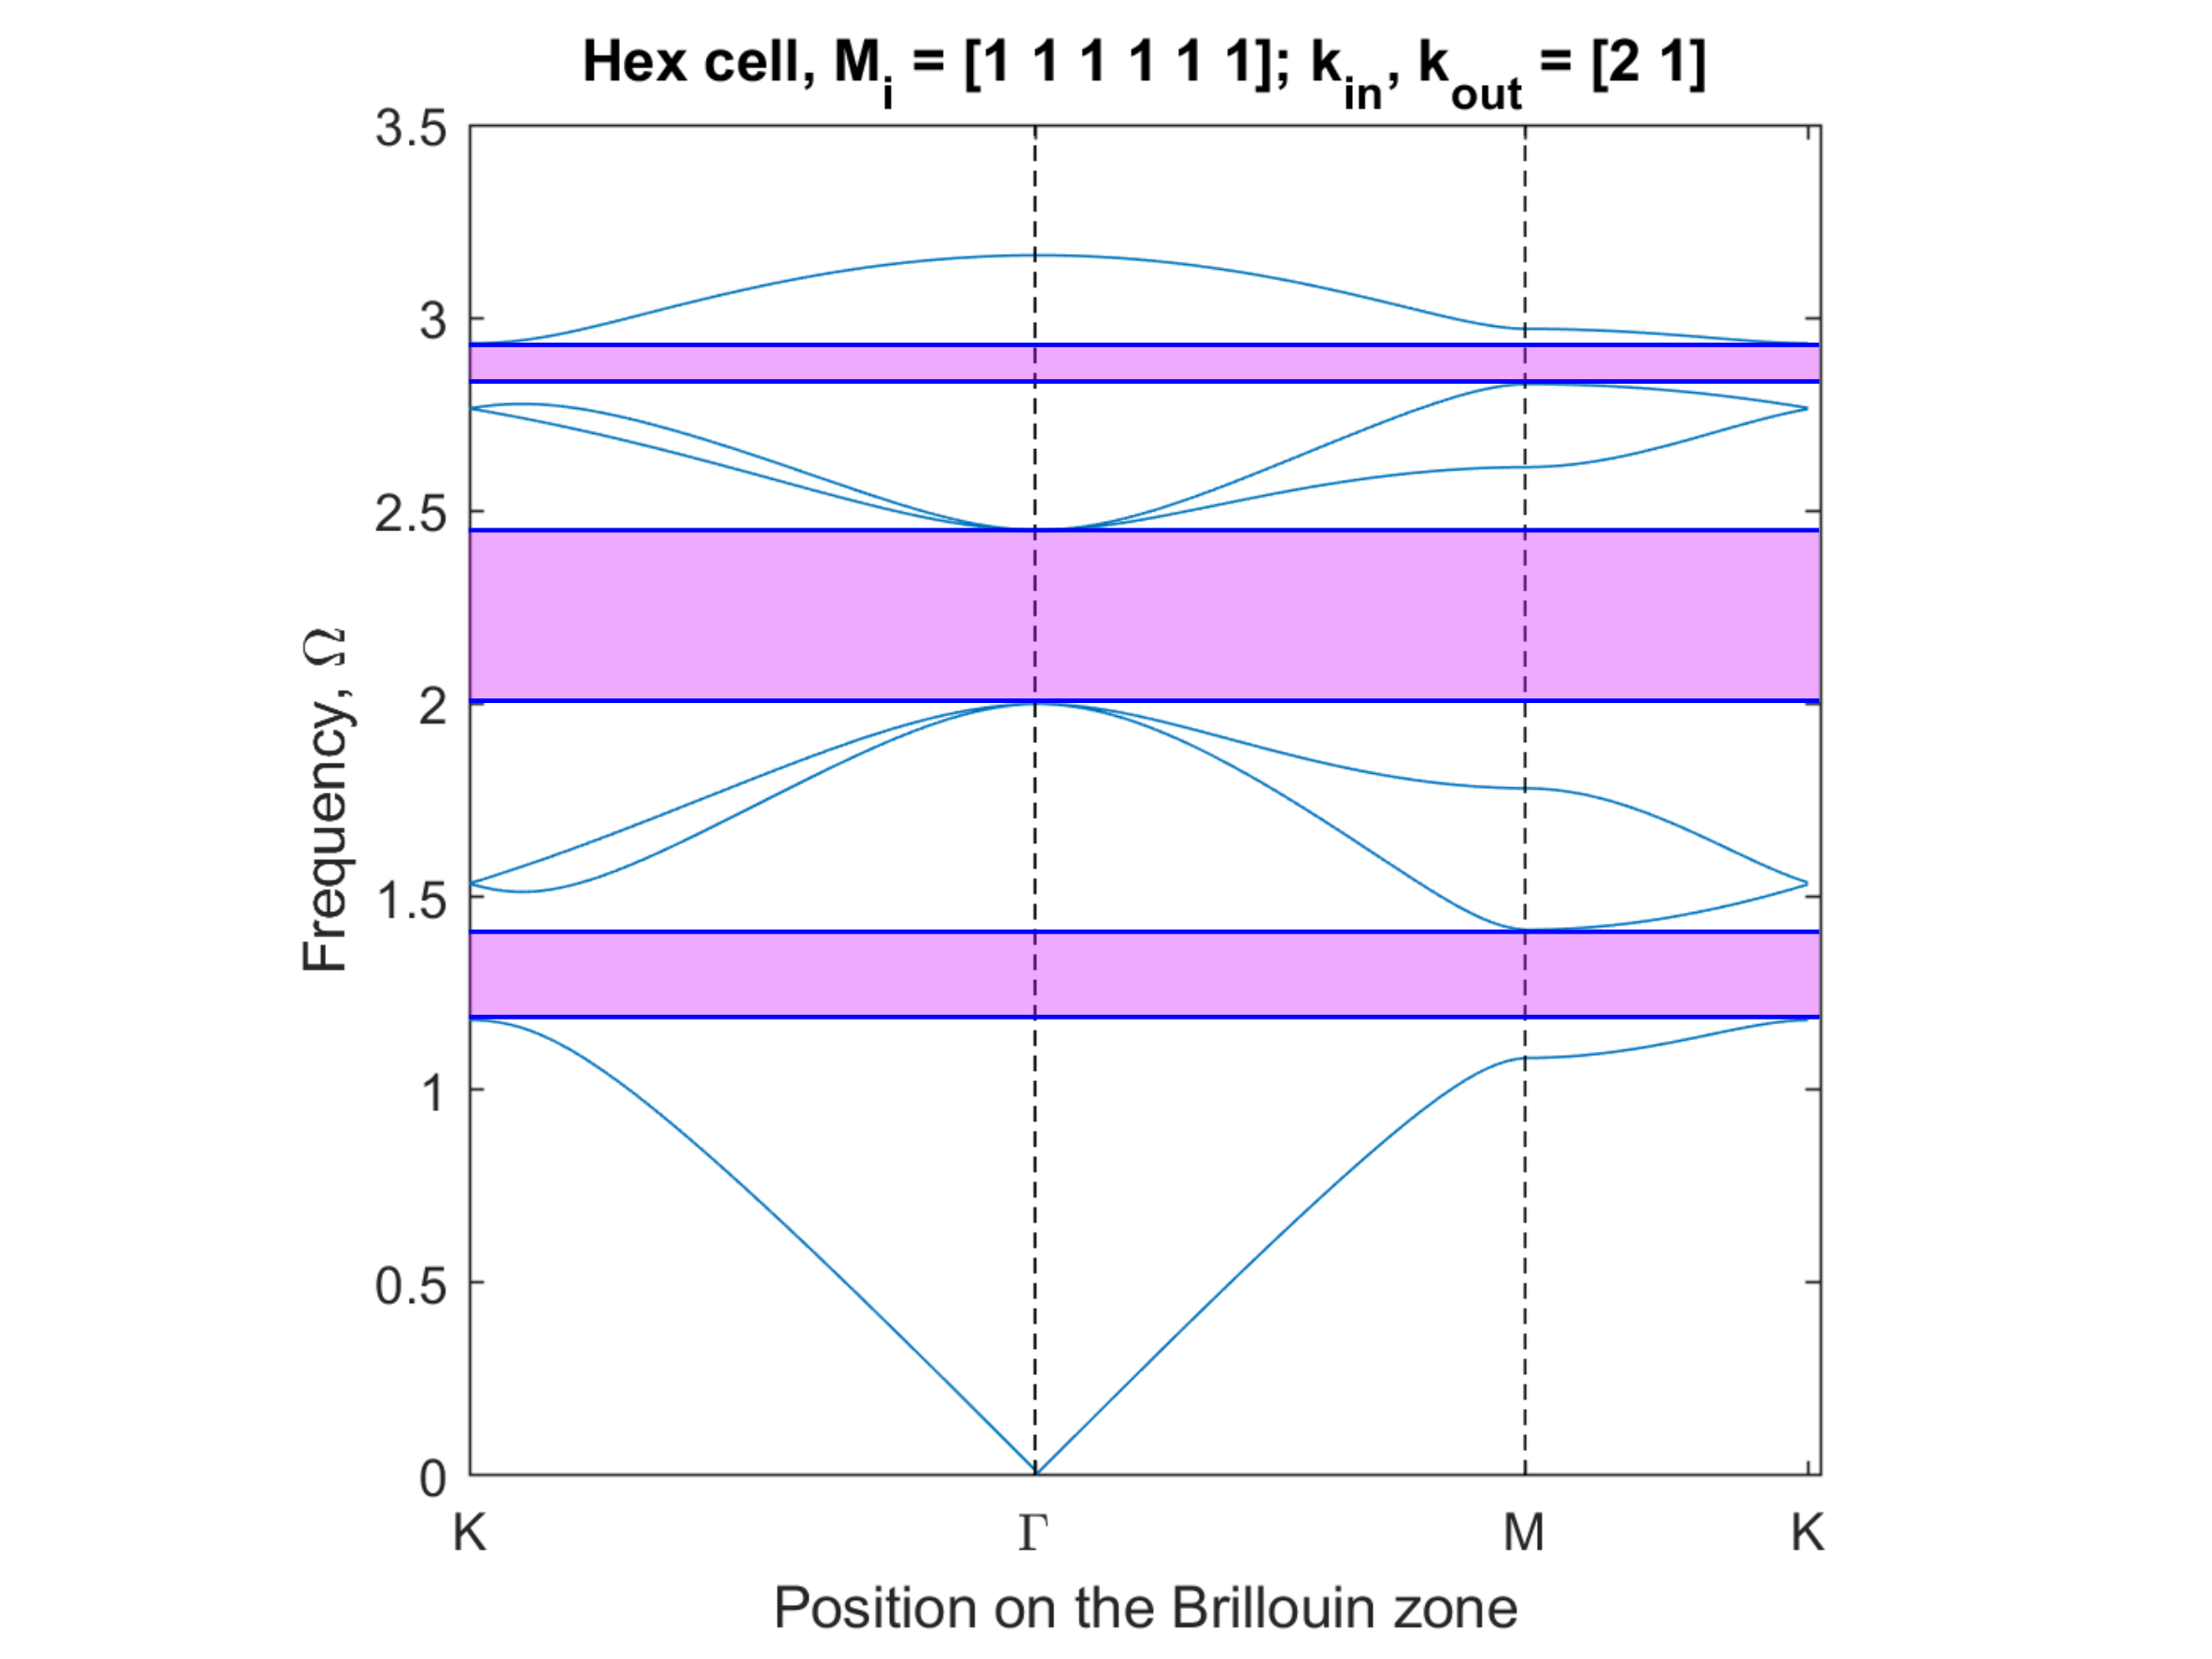
\includegraphics[width=0.8\textwidth]{imgs/bandgapex.png}
\caption{\label{fig:bandgapex} Example of bandgap (purple) formed in dispersion
  relation of hex lattice when $k=2$ and $\tilde{k}=1$.}
\end{figure}

A band gap, also called an energy gap, is an energy range where no wave states
can exist. In terms of our lattices, this corresponds to a range of frequencies
where waves are unable to propagate through the material; and in graphs of
dispersion relations, it is seen as gaps in the frequency axis where no line
is present. An example is shown in Figure~\ref{fig:bandgapex}. 
%TODO: What is a bandgap?

%TODO: Form bandgaps for hex and kagome cell
\section{2d bulk hexagonal perturbation}
One way to perturb our bulk hexagonal lattice is by breaking one of its
rotational symmetries. Currently our hexagonal lattice has six-fold rotational
symmetry, i.e. rotating our cells by $\frac{2pi}{6}$ do not change them. We can
reduce this to a three-fold symmetry by alternating the masses such that
$M_1=M_3=M_5 \neq M_2=M_4=M_6$.

\begin{figure}[!h]
\centering
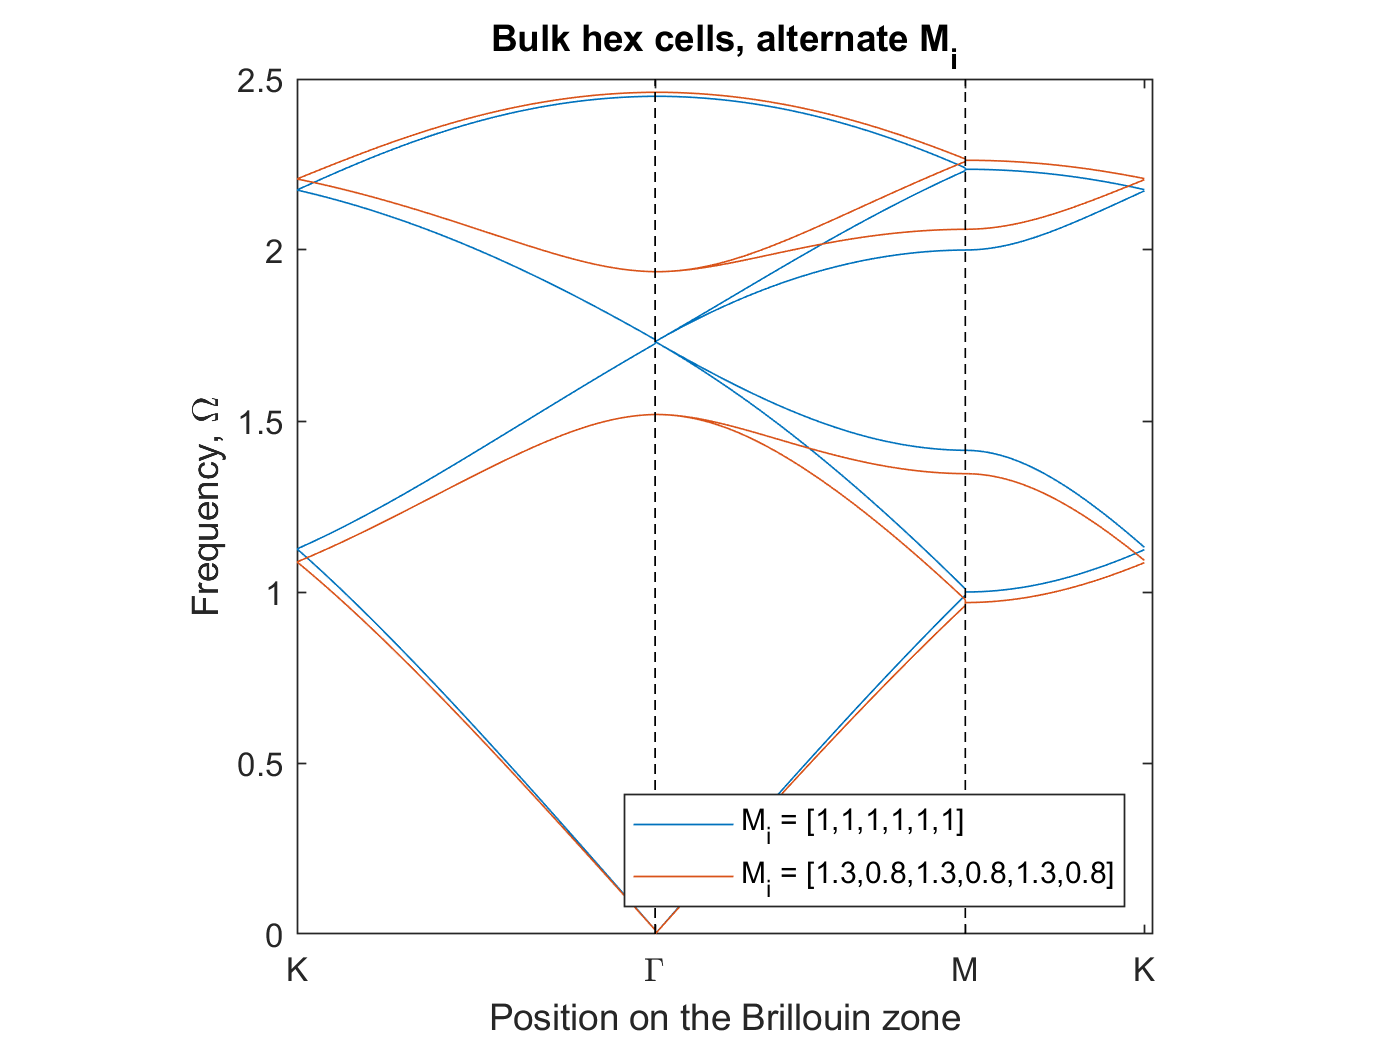
\includegraphics[width=0.8\textwidth]{imgs/hexperturbM.png}
\caption{\label{fig:hexM} The effect of alternating the masses $M_i$ on the
  dispersion relation of the bulk hexagonal system, with all other parameters
  set to $1$.}
\end{figure}

In Figure~\ref{fig:hexM}, we see that alternating masses has opened up the
double dirac point at $\Gamma$ and formed a bandgap.

\section{2d bulk kagome perturbation}
Similarly to the hexagonal case, we can perturb the different parameters in our
bulk kagome system to see what effects they have on the dispersion relation.

\begin{figure}[!h]
\centering
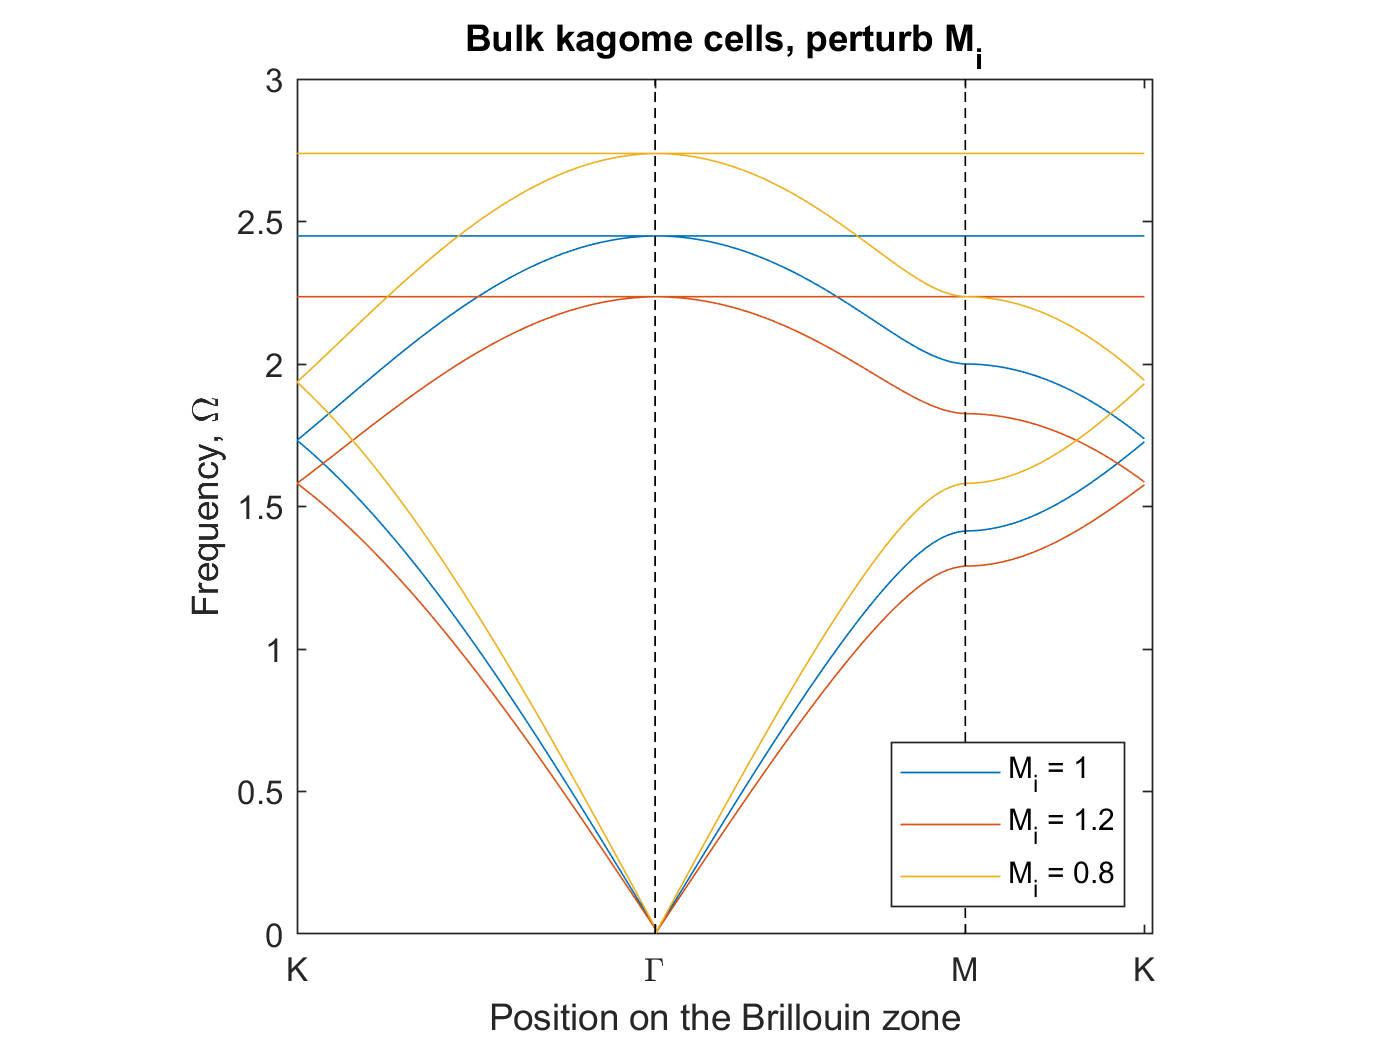
\includegraphics[width=0.8\textwidth]{imgs/kagomeperturbM.png}
\caption{\label{fig:kagomeM} The effect of perturbing the mass $M$ on the
  dispersion relation of the bulk kagome system, with all other parameters set
  to $1$.}
\end{figure}

\begin{figure}[!h]
\centering
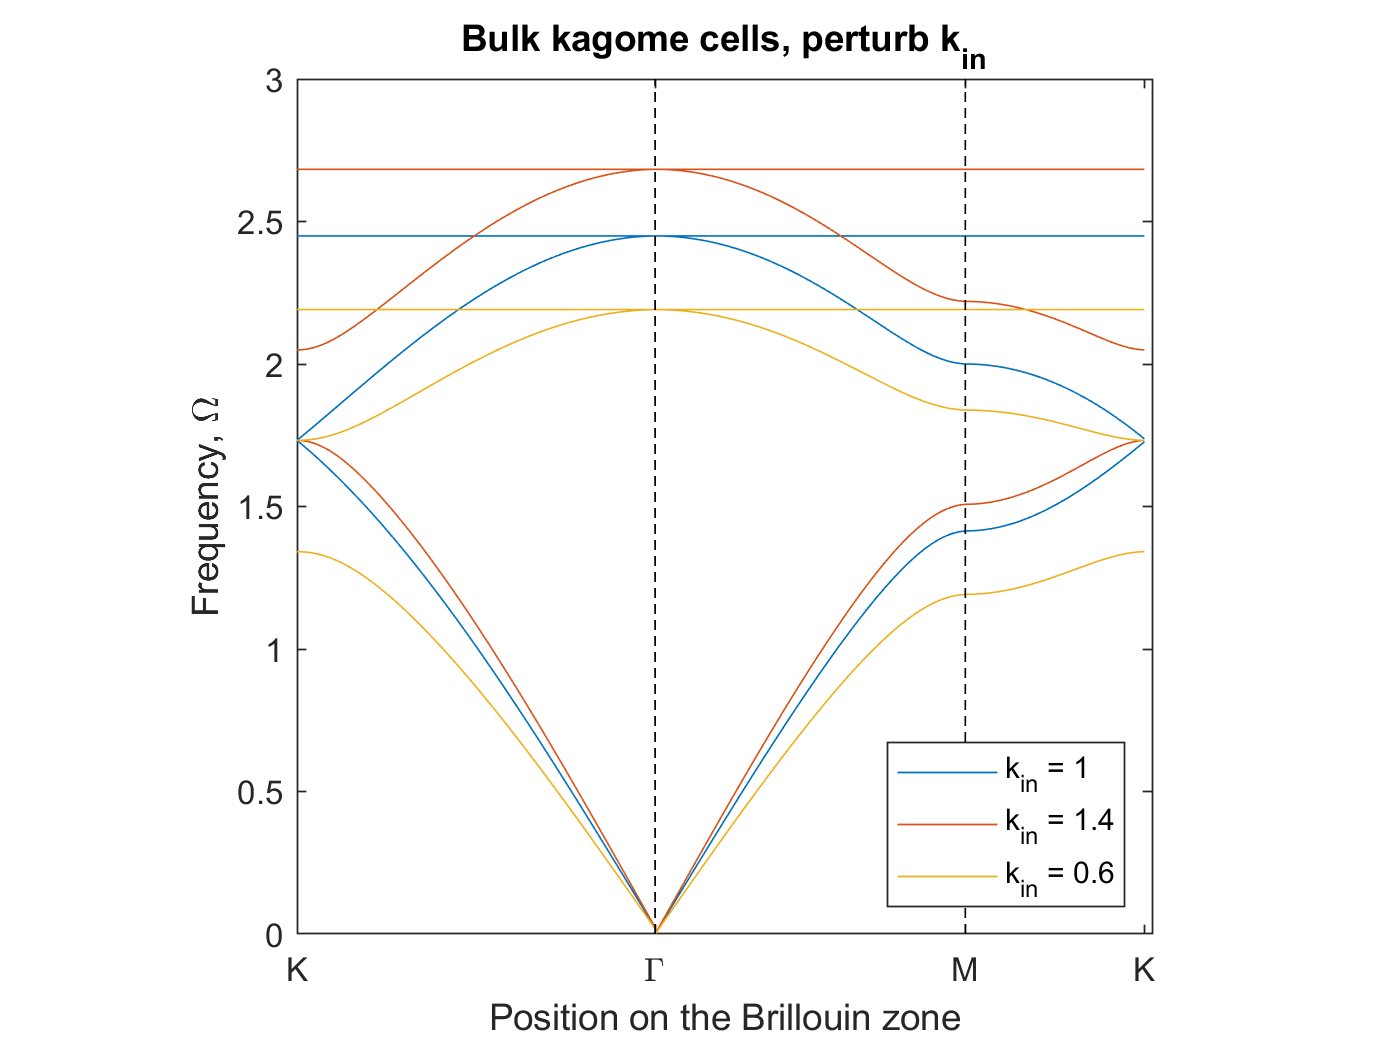
\includegraphics[width=0.8\textwidth]{imgs/kagomeperturbk.png}
\caption{\label{fig:kagomek} The effect of perturbing the inner stiffness $k$
  on the dispersion relation of the bulk kagome system, with all other
  parameters set to $1$.}
\end{figure}

We can see the effects that perturbing the mass $M$ and inner stiffness $k$
have on the bulk kagome system. In the case of varying $M$ in
Figure~\ref{fig:kagomeM}, increasing $M$ decreases or constrains the dispersion
relation, while decreasing $M$ increases or widens the dispersion relation. 

However, in the case of varying $k$ in Figure~\ref{fig:kagomek}, we see the inverse
effect; increasing $k$ increases or widens the dispersion relation, while
decreasing $k$ decreases or constrains the dispersion relation. Another
interesting thing to notice about changing $k$ is that it causes the formation
of a bandgap!

With these two inverse relationships, we are naturally propelled to ask what
happens if we combine both of these effects together. For example, by
increasing $M$ and increasing $k$, would the two effects \textit{cancel out} to
give us the same dispersion relation as the unperturbed system?

\begin{figure}[!h]
\centering
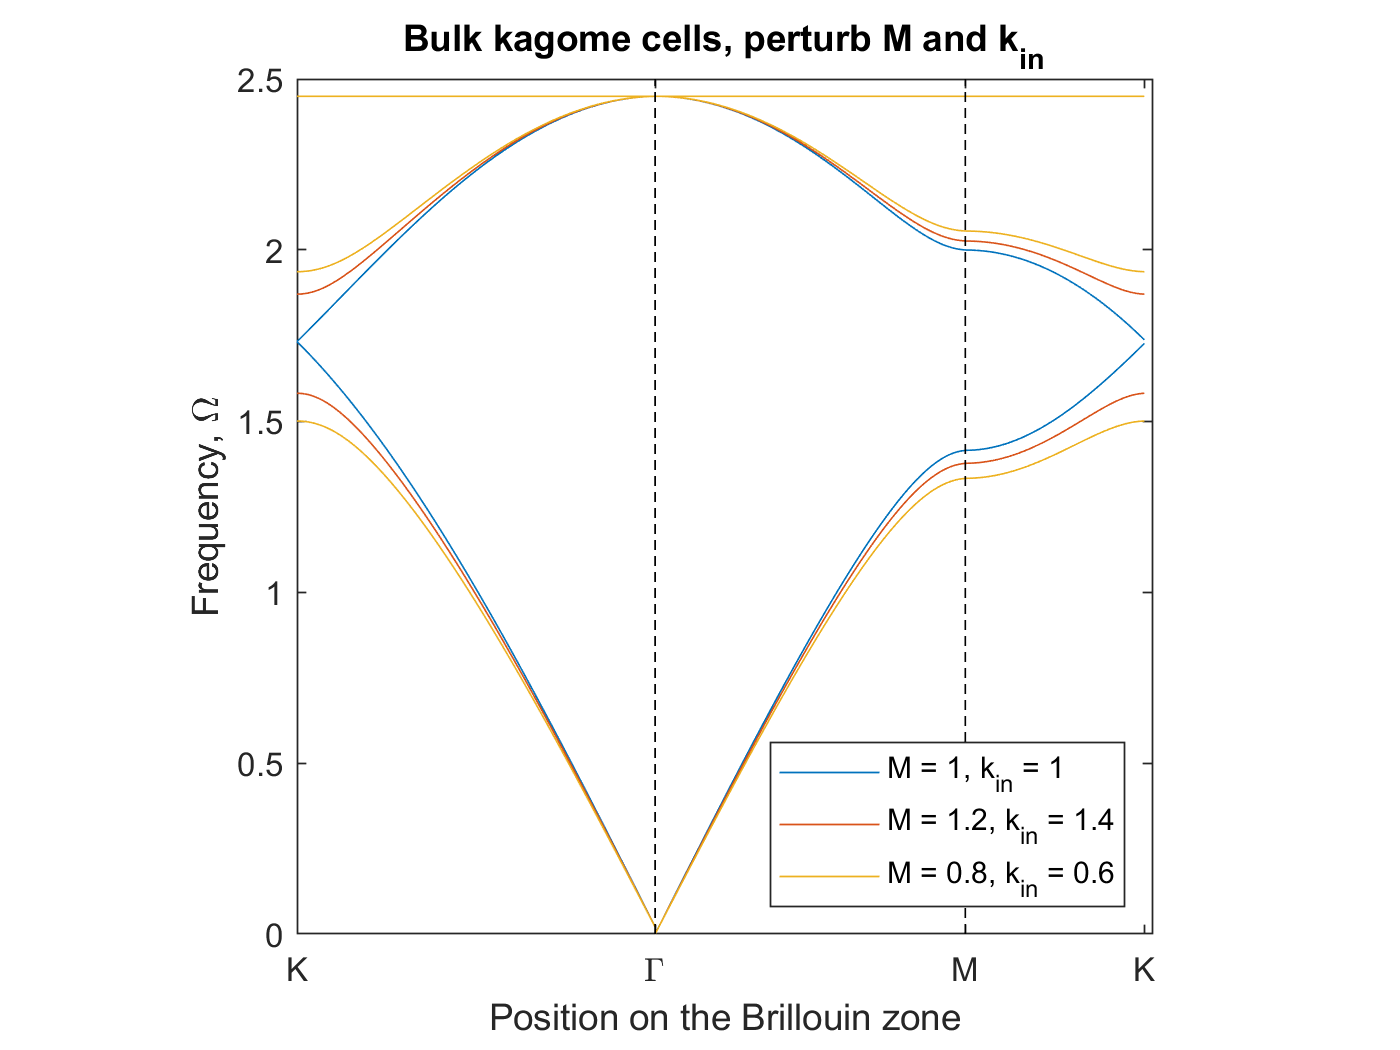
\includegraphics[width=0.8\textwidth]{imgs/kagomeperturb2.png}
\caption{\label{fig:kagome2} The effect of perturbing both the mass $M$ and the
  inner stiffness $k$ on the dispersion relation of the bulk kagome system,
  with all other parameters set to $1$.}
\end{figure}

\section{Band gap inversion}
%TODO: Decide if want to include

\section{2d hexagonal strip}
\label{formstrip}
%TODO: How does bandgap relate to the dispersion along the boundary?

\begin{figure}[!h]
\centering
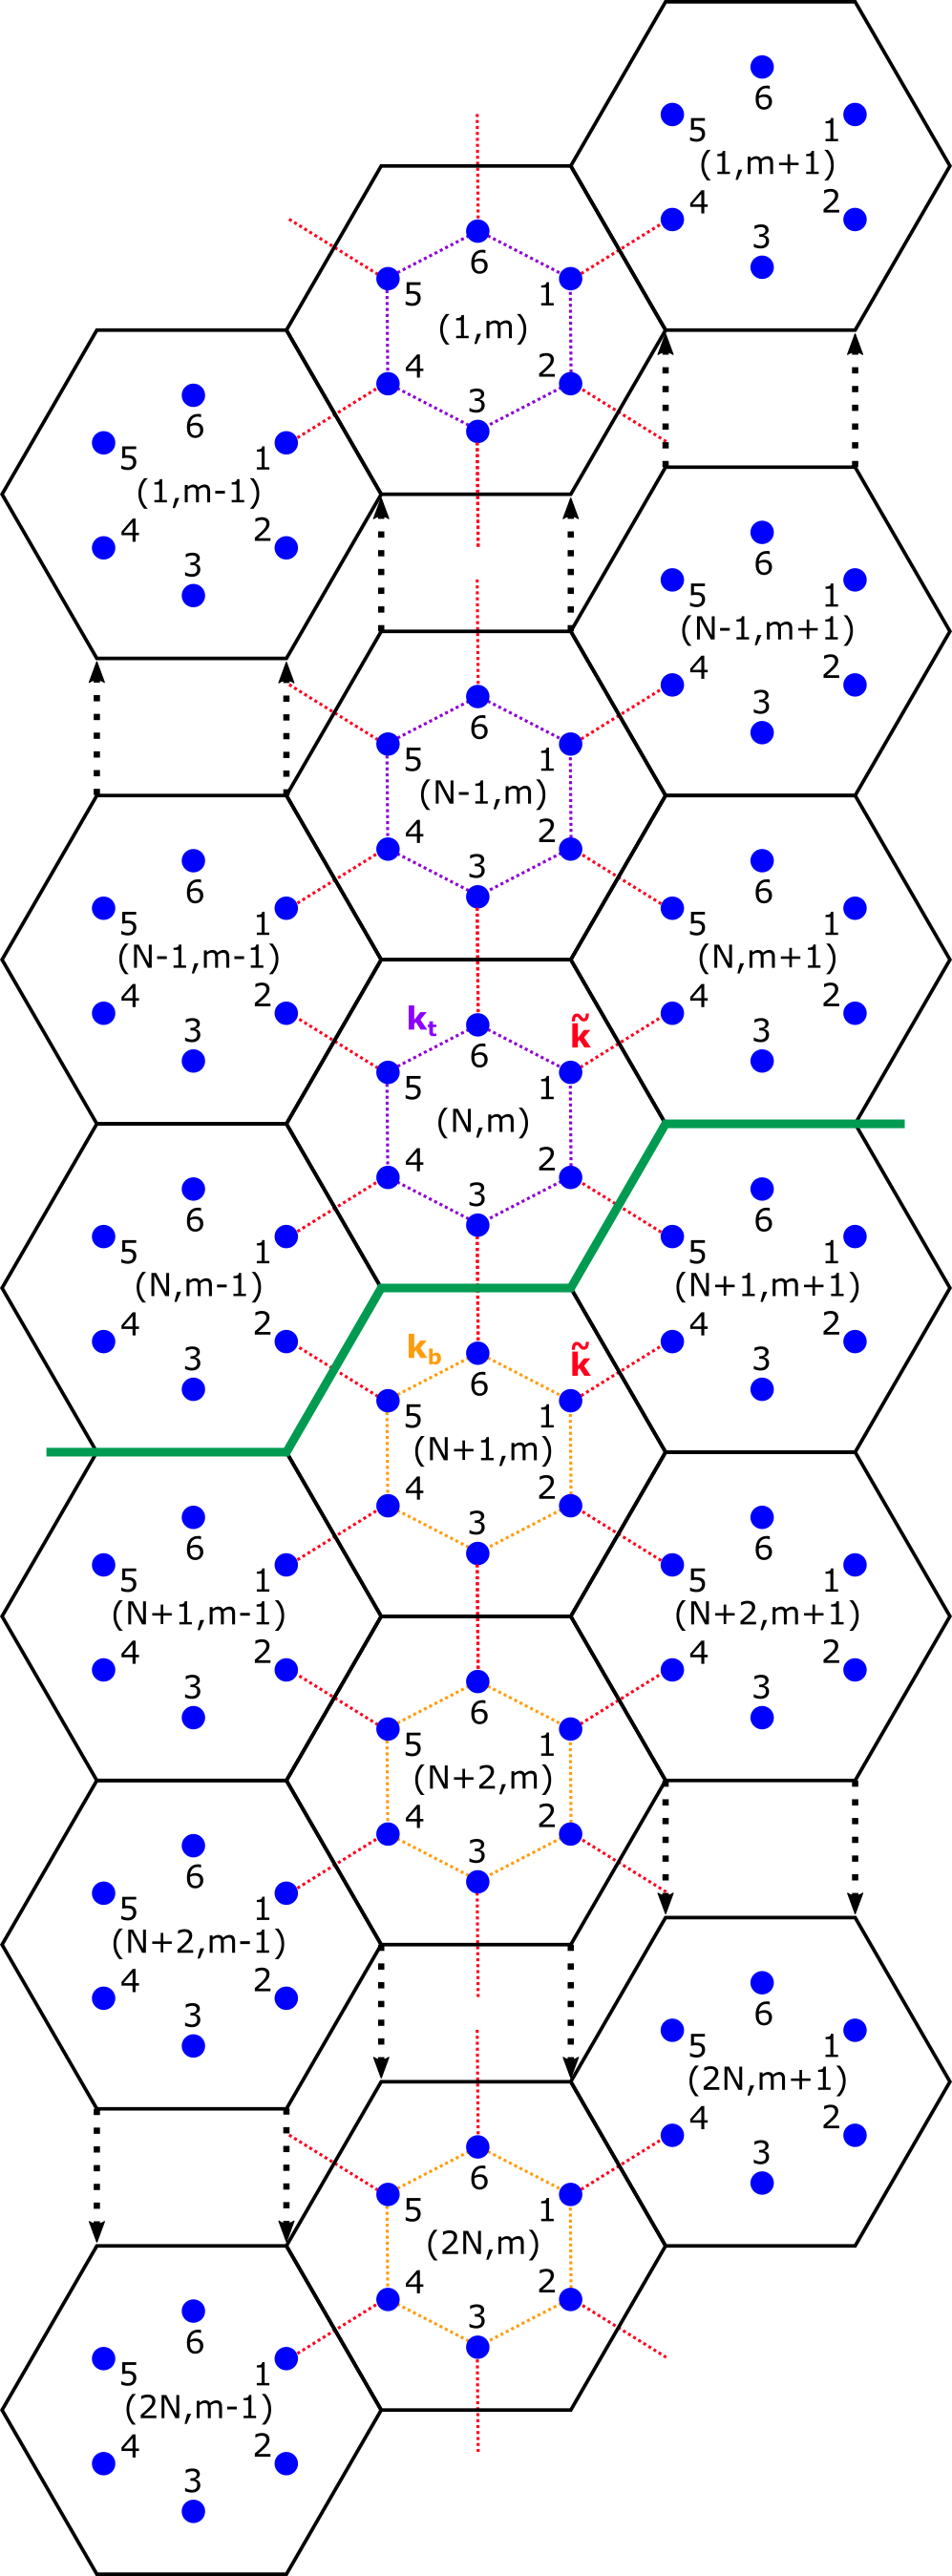
\includegraphics[width=0.4\textwidth]{imgs/hexstripmodel.png}
\caption{\label{fig:hexstripmodel} Schematic view of the 2d hexagonal
  semi-infinite lattice made from an infinite number of strips connected
  side-by-side. Each strip is composed of 2N cells, with the top half of cells
  above the boundary (green) possessing a set of properties and the bottom half
  possessing a separate set of properties.}
\end{figure}

Now we assemble $2N$ hexagonal cells together into a strip. We will subscript
the values corresponding to the top half and bottom half with $t$ and $b$
respectively, e.g. $k_t$ to refer to the inner spring constants for the top
half and $M_{1,b}$ to refer to the mass of mass $1$ in the bottom half. We set
the outer spring constant, $\tilde{k}_t=\tilde{k}_b=\tilde{k}$ to be the same
throughout the strip, to ensure that it agrees on both sides of the boundary or
interface.

\section{2d kagome strip}
%TODO: Derive IBZ

\begin{figure}[!h]
\centering
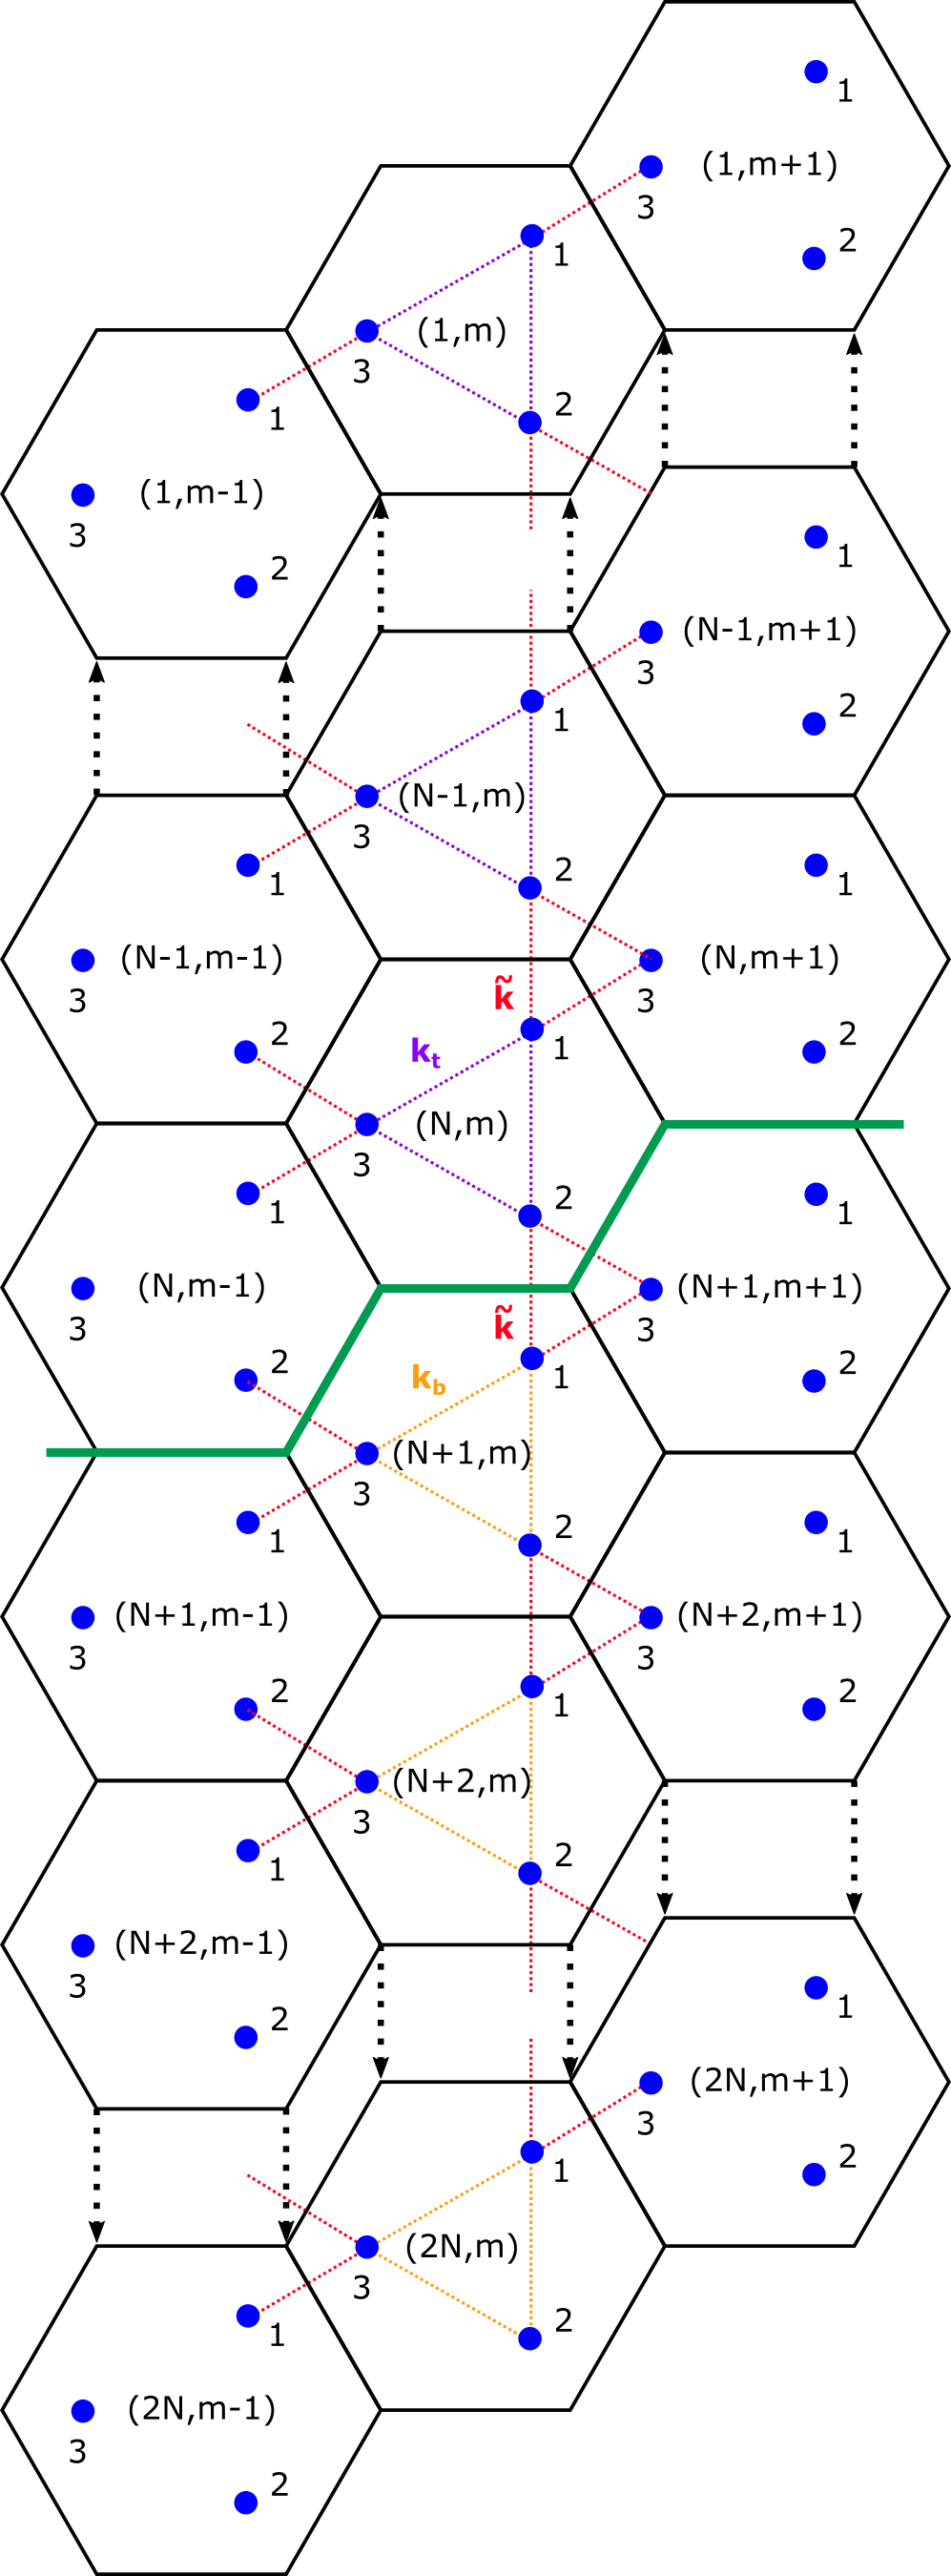
\includegraphics[width=0.4\textwidth]{imgs/kagomestripmodel.png}
\caption{\label{fig:kagomestripmodel} Schematic view of the 2d kagome
  semi-infinite lattice made from an infinite number of strips connected
  side-by-side. Each strip is composed of 2N cells, with the top half of cells
  above the boundary (green) possessing a set of properties and the bottom half
  possessing a separate set of properties.}
\end{figure}

Using the same conventions as the hexagonal strip case, we form the eigen-problem 

\begin{align}
  \left[\matr{A}\left(\kappa_{x},\kappa_{y}\right)-\matr{\Omega}\matr{M}\right]\vec{y}=\vec{0}
\label{eq:kagomestripeig}
\end{align}

where $\matr{\Omega}=\diag\left(\left\{\Omega_i^2\right\}\right)$,
$\matr{M}_{t}=\diag\left(\left\{M_{i,t}\right\}\right)$,
$\matr{M}_{b}=\diag\left(\left\{M_{i,b}\right\}\right)$,
\begin{align}
\matr{M}=\left[
\begin{array}{cccccc}
\matr{M}_{t}\\
 & \ddots &  &  & 0\\
 &  & \matr{M}_{t}\\
 &  &  & \matr{M}_{b}\\
 & 0 &  &  & \ddots\\
 &  &  &  &  & \matr{M}_{b}
\end{array}\right],
\end{align}

\begin{align}
\vec{y}=\left[
\begin{array}{c}
y_1^{(1)}\\
y_2^{(1)}\\
y_3^{(1)}\\
\vdots\\
y_1^{(2N)}\\
y_2^{(2N)}\\
y_3^{(2N)}\\
\end{array}\right],
\end{align}

\begin{align}
  \matr{A}\left(\kappa_{x},\kappa_{y}\right)=\left[
\begin{array}{ccc}
2k+2\tilde{k} & -k-\tilde{k}e^{-i\Delta_3} & -k-\tilde{k}e^{i\Delta_1} \\
-k-\tilde{k}e^{i\Delta_3} & 2k+2\tilde{k} & -k-\tilde{k}e^{i\Delta_2} \\
-k-\tilde{k}e^{-i\Delta_1} & -k-\tilde{k}e^{-i\Delta_2} & 2k+2\tilde{k} 
\end{array}\right]
\end{align}
%TODO: Fix A

Solving this with $M_{i,t}=M_{i,b}=k_t=k_b=\tilde{k}=1$ over the irreducible
Brilloun zone gives us the dispersion relation in
Figure~\ref{fig:kagomestripdisper}.

\begin{figure}[!h]
\centering
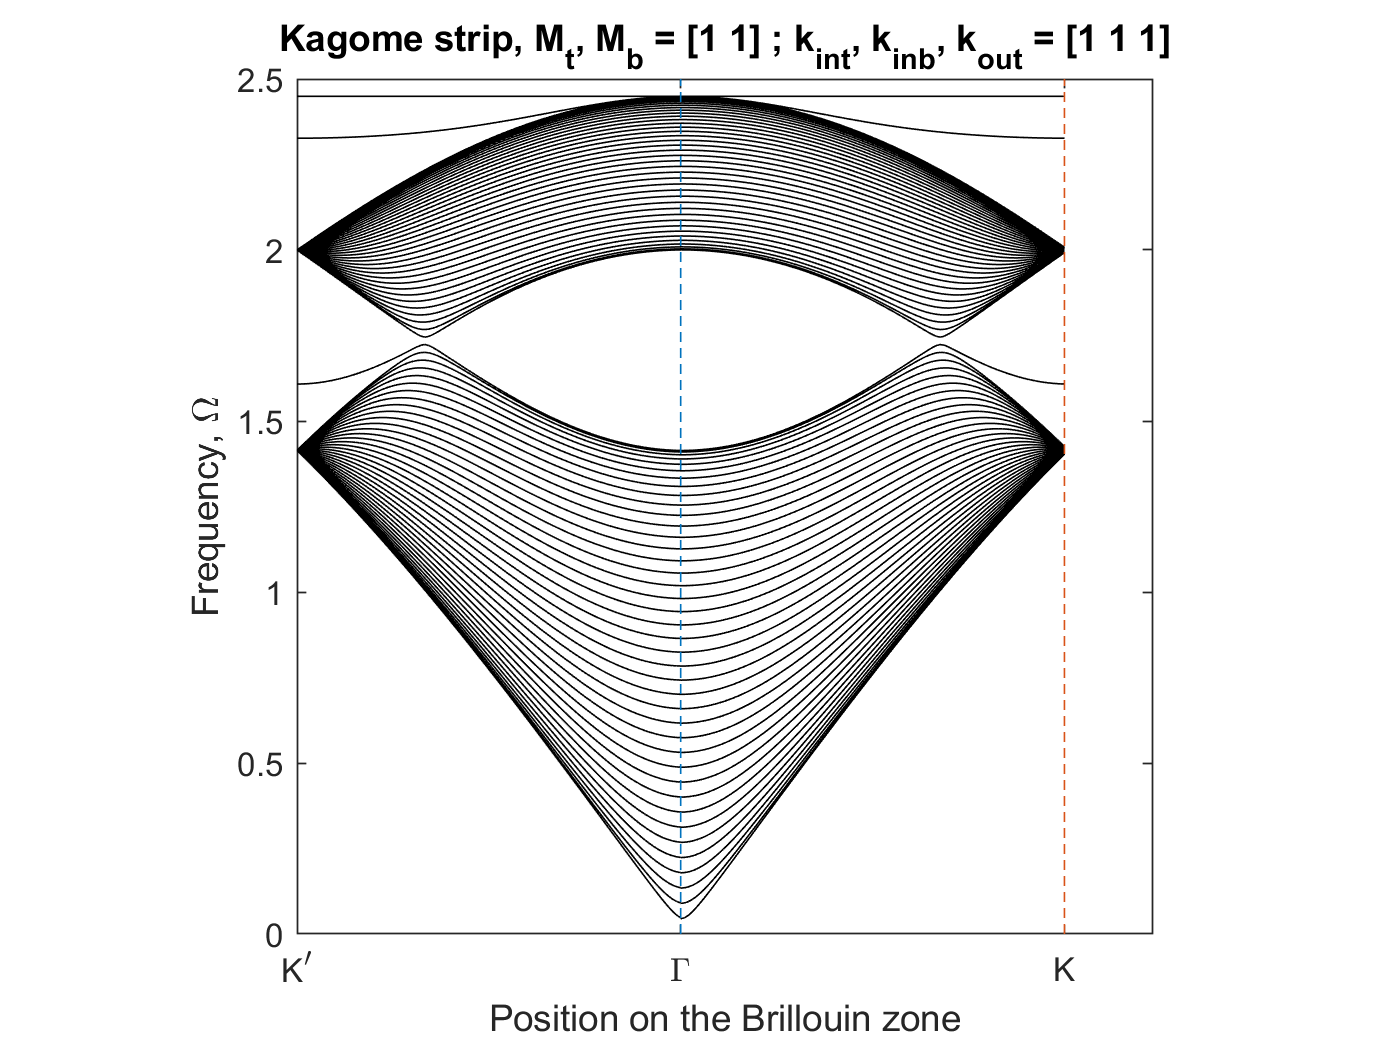
\includegraphics[width=0.8\textwidth]{imgs/kagomestrip.png}
\caption{\label{fig:kagomestripdisper} Dispersion relation of a kagome strip
  with $N=40$ (80 cells in total) with $M_{i,t}=M_{i,b}=k_t=k_b=\tilde{k}=1$.}
\end{figure}


